% ======================================================================
\section{The LunarSim-VPR Benchmark}\label{sec:bench}
% ======================================================================
No public lunar surface dataset combines dense pose ground truth with systematic illumination
coverage. We therefore built a lightweight, reproducible renderer that targets the three properties
that make lunar VPR hard: self-similar relief, hard shadows and non-Lambertian photometry. It does
not replace real data (\cref{sec:limits}), but it lets us vary one factor at a time with exact
ground truth. It complements DESPINA~\cite{nelsonarcher2026despina}, which produces realistic
appearance for real sites from LRO DEMs but does not expose explicit control of the Sun direction.

\paragraph*{Terrain}
Each scene combines a \emph{regional} DEM ($16$\,m/px, $16.4$\,km) and a \emph{local} DEM
($0.3$\,m/px, $614$\,m) blended into its centre. Both start from fractional-Brownian relief
(power spectrum $\propto k^{-\beta}$, $\beta\in[2.2,3.2]$). Craters are drawn from an
equilibrium-like cumulative size--frequency distribution $N(>D)=cD^{-2}$~\cite{melosh1989impact}
($D\in[60,2500]$\,m regionally and $[1.5,120]$\,m locally) and stamped with a bowl--rim--ejecta
profile whose depth-to-diameter ratio ($0.04$--$0.2$) and rim height depend on a random degradation
state. Fresh craters get bright albedo halos and ejecta boulders. Four to seven distant massifs
($200$--$700$\,m high, $4$--$7.5$\,km away) give a horizon silhouette, as at the Apollo~17 site
(\cref{fig:apollo}).


\begin{figure}[t]
\centering
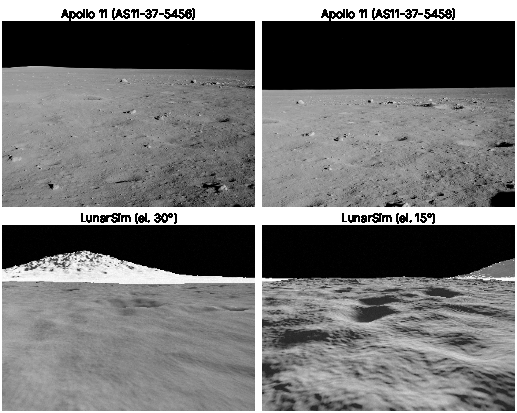
\includegraphics[width=\columnwidth]{figures/apollo_vs_sim.pdf}
\caption{Real Apollo~11 surface photographs~\cite{apollo11} (top) and LunarSim renders (bottom).
The renderer reproduces the black sky, the horizon structure and the shading statistics of
low-Sun regolith. It under-resolves near-field rocks smaller than the $0.3$\,m DEM spacing, a
limitation discussed in \cref{sec:limits}.}
\label{fig:apollo}
\end{figure}

\paragraph*{Photometry and shadows}
Radiance follows the lunar-Lambert function of McEwen~\cite{mcewen1991photometric},
$I\propto A\,[2L(g)\cos i/(\cos i+\cos e)+(1-L(g))\cos i]$, with phase-dependent $L(g)$. It is
multiplied by a Hapke-style shadow-hiding opposition term
$1+B_0/(1+\tan(g/2)/h)$~\cite{hapke2012theory}, where $i$, $e$ and $g$ are the incidence, emission and
phase angles. Cast shadows are computed from both DEMs (so massifs shade the valley at low Sun),
averaged over the $0.53^\circ$ solar disk to produce penumbrae. A weak ambient term models
earthshine and inter-reflection, and a footprint-faded micro-relief bump map adds sub-grid regolith
texture.

\paragraph*{Camera}
A rover-mounted pinhole camera ($70^\circ$ HFOV, $320\times240$, $1.35$--$1.7$\,m high) is rendered
by column-wise height-field ray casting, accounting for lunar curvature. The renderer applies
centre-weighted auto-exposure, a soft-shoulder tone curve, gamma, shot and read noise, and 8-bit
quantisation. One image takes about $0.15$\,s on a CPU once the shadow maps for a Sun direction
have been computed.

\paragraph*{Protocol}
Each scene contains a smooth random traverse with places every $6$\,m. The database is rendered at
one Sun direction (azimuth $135^\circ$, elevation $30^\circ$). Queries are taken at jittered poses
(up to $3$\,m offset, $\mathcal{N}(0,10^\circ)$ heading noise, random camera height). The
\emph{same} query poses are rendered under seven Sun conditions (\cref{tab:conds}), so differences
between conditions are paired and caused by illumination alone. The test set has three unseen
scenes ($3\times150$ database images and $3\times1050$ queries), the validation set one scene
($100$ places, $700$ queries), and the training set five further scenes with $240$ places $\times$
$4$ views. Training views use Sun directions drawn from a per-scene pool of $16$ random
directions (elevation $4^\circ$--$75^\circ$, any azimuth), which mimics an illumination-sweep
dataset.

\begin{table}[t]
\centering
\caption{Query illumination conditions (Sun azimuth/elevation in degrees). The database is rendered at
azimuth $135^\circ$, elevation $30^\circ$.}
\label{tab:conds}
\scriptsize
\setlength{\tabcolsep}{3pt}
\begin{tabular}{@{}lccccccc@{}}
\toprule
 & C0 & C1 & C2 & C3 & C4 & C5 & C6 \\
\midrule
Az./El. & 135/30 & 135/15 & 135/6 & 135/60 & 225/30 & 315/30 & 315/8 \\
Change & view & lower & grazing & high & rot.\ $90^\circ$ & flip & flip+graz.\ \\
\bottomrule
\end{tabular}
\end{table}
